\chapter{\IfLanguageName{dutch}{Selecteren frameworks}{Selecting frameworks}}
\label{ch:selecteren-frameworks}

In het vorige hoofdstuk werden de eisen gedefiniëerd waaraan de frameworks binnen deze studie moeten voldoen. In dit hoofdstuk worden alle populaire cross-platform frameworks opgesomd en vervolgens afgetoetst tegen deze eisen. Enkel de frameworks die voldoen aan al deze eisen worden verder in deze studie nog behandeld, de andere frameworks liggen buiten het doel van deze studie. 

Om tot een lijst van de populairste frameworks te komen werd gekeken naar de resultaten van een wereldwijde ondervraging door JetBrains \autocite{Liu2020}. Met 19696 deelnemers aan deze ondervraging is dit een zeer goede weergave van de populariteit van de verschillende frameworks onder ontwikkelaars. In de volgende sectie worden de populairste cross-platform frameworks uit deze ondervraging opgesomd. In een volgend hoofdstuk worden deze frameworks vervolgens afgetoetst tegen de gestelde eisen.

\section{Populairste cross-platform frameworks}

In figuur \ref{fig:frameworkPopularity} zijn de resultaten van de ondervraging door JetBrains te zien. Uit deze figuur blijkt dat er enkele zeer populaire frameworks zijn, waarvan React Native en Flutter de populairste zijn. Een interessante opmerking is dat de populariteit van Flutter sterk gestegen is (+9\%) in 2020 in vergelijking met 2019, waar die van React Native hetzelfde gebleven is (42\%). Anderzijds is de populariteit van enkele andere frameworks sterk gedaald: Cordova (-11\%), Ionic (-10\%) en Xamarin (-12\%) zijn een heel pak gebruikers kwijt geraakt. Tot slot zijn helemaal rechts enkele frameworks te zien die in 2019 door geen enkele van de ondervraagden gebruikt werden maar in 2020 wel een bepaald (weliswaar laag) percentage gebruikers weten te overtuigen. Zo duikt bijvoorbeeld Kotlin Multiplatform op in de ondervraging, met 2\% van de ondervraagden die aangeven dit te gebruiken. Ook Kivy en Corona duiken op in de resultaten van de ondervraging in 2020 met elk 1\% van de ondervraagden die aangeeft er gebruik van te maken.

Alle frameworks die aan bod komen in deze ondervraging zullen in de volgende sectie kort besproken worden en vervolgens afgetoetst worden tegen de gestelde eisen. Het is namelijk niet automatisch zo dat het (op dit moment) populairste framework ook meteen de beste keuze is voor de komende jaren.

\begin{figure}
    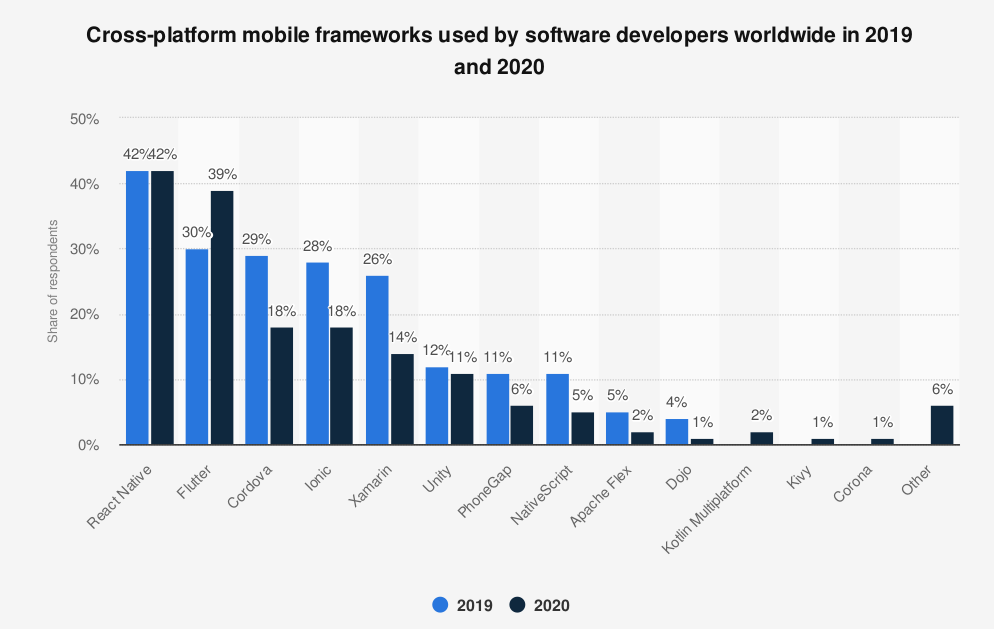
\includegraphics[width=\linewidth]{PopularFrameworksGraph.png}
    \caption{Resultaten van de populariteitsondervraging van cross-platform frameworks door JetBrains}
    \label{fig:frameworkPopularity}
\end{figure}

\section{Achtergrond frameworks en aftoetsing tegen eisen}

In deze sectie wordt de achtergrondinformatie van alle frameworks die aan bod komen in de ondervraging van JetBrains kort besproken. Vervolgens worden ze één voor één afgetoetst aan de in hoofdstuk \ref{ch:eisen-framework} gestelde eisen. De frameworks die aan alle eisen voldoen worden vervolgens uitgebreid voorgesteld in hoofdstuk ... 

\subsection{React Native}

React Native (2015) is een open source cross platform framework dat ontwikkeld is en onderhouden wordt door Facebook \autocite. Zoals de naam al doet vermoeden steunt dit framework op React (een Javascript library, ook ontwikkeld door Facebook). React is speciaal ontwikkeld om gebruikersinterfaces te maken, maar waar React zelf zich richt op webbrowsers focust React Native zich op mobiele platformen. Met behulp van React Native kunnen applicaties geschreven worden die er helemaal native uitzien en dit in een taal die reeds heel erg gekend is onder ontwikkelaars \autocite{Eisenman2015}.

\subsection{Flutter}

Flutter is een software development kit (SDK) ontwikkeld door Google in 2017. Het is een 'UI toolkit' om native gecompileerde apps te maken die er mooi uizien met een enkele broncode \autocite{Google2020}. Net zoals React Native is ook Flutter volledig open source. Het kan rekenen op een grote community en voortdurende verdere ontwikkeling. De laatste stabiele versie van Flutter werd uitgebracht door Google op 6/5/2020. Het is dus een zeer recente update waardoor de SDK kan rekenen op de laatste nieuwe ontwikkelingen op het vlak van cross platform development. Flutter apps worden geschreven in Dart, een object georiënteerde programmeertaal gebaseerd op klassen en ontwikkeld door Google. Het grote voordeel van Dart is dat het gecompileerd kan worden naar Javascript maar ook rechtstreeks naar native code, wat een groot voordeel oplevert op het vlak van prestaties.



